%!TEX program = xelatex
\documentclass[12pt,a4paper]{article}

\usepackage{amssymb}
\usepackage{amsmath}
\usepackage{amsthm}
\usepackage{mathtools}
\usepackage{clrscode3e}
\usepackage{graphicx}
\usepackage{listings}
\usepackage{subfig}
\usepackage{listing}
\usepackage{enumitem}
\usepackage{hyperref}
\usepackage{url}
\usepackage{tcolorbox}
\usepackage{tikz}
\usepackage{tabularx}
\usepackage{array}
\usepackage{enumitem}
\usepackage{setspace}
\usepackage{verbatim}
\newcolumntype{C}{>$c<$}
\lstset{basicstyle=\ttfamily}
\usetikzlibrary{calc,shapes.multipart,chains,arrows}
\newcommand{\points}[1]{ ($#1$ \textit{points}) } 
\newcommand{\xor}{\oplus} 
\newcommand{\bigxor}{\bigoplus} 
\usepackage{xeCJK}
\setCJKmainfont{AR PL UKai TW}

\usepackage{fontspec}
%\setmainfont{Gill Sans MT}
%\setmainfont{Helvetica}

\pagestyle{plain}

\setlength{\parskip}{10pt}
\fontsize{12}{14}
\selectfont
\textwidth=17cm \textheight=24cm \voffset=-2cm \hoffset=-1.7cm

\makeatother
\newcommand{\fontitem}{\Large}
\newcommand{\fontitemi}{\normalsize}
\newcommand{\fontitemii}{\normalsize}
\newcommand{\flag}[1]{\\\hfill\footnotesize\lstinline|BALSN\{#1\}|}

\DeclarePairedDelimiter\ceil{\lceil}{\rceil}
\DeclarePairedDelimiter\floor{\lfloor}{\rfloor}

\def\headline#1{\hbox to \hsize{\hrulefill\quad\lower.3em\hbox{#1}\quad\hrulefill}}
\def\headline#1{\hbox to \hsize{\hrulefill\quad\lower.3em\hbox{#1}\quad\hrulefill}}

\begin{document}

\begin{center}
\textbf{\Large Theory of Computer Games, Fall 2018\\}
\textbf{\Large Homework 2\\} 
\vspace{5pt}
\textbf{B04902012 Han-Sheng Liu, CSIE, NTU}\\
E-mail: \href{mailto:b04902012@ntu.edu.tw}{\texttt{b04902012@ntu.edu.tw}}\\

\end{center}
\vspace{5pt}
\section{Compilation}
\texttt{g++ b04902012.cpp -O2 -o b04902012}
\section{Execution}
\lstinline{./b04902012}
\section{Implementation}
    \subsection{Encode/Hash}
        一個盤面是由 5$\times$5 的棋盤,以及若干個棋子組成。其中,棋子可以分成四類:
        \begin{itemize}
        \item \(A\): 本回合可移動的棋子
        \item \(B\): 下回合可移動的棋子
        \item \(C\): 下下回合可移動的棋子
        \item \(D\): 下下下回合可移動的棋子
        \end{itemize}
        如果有兩個盤面,它們的四種棋子的位置分佈都相同,那麼它們便應該被等價地看待。注意到位置是以「該回合的玩家」的視角為準,而不是棋盤的絕對位置。
        對於紅色玩家和藍色玩家,可以分別把 25 個格子以對稱的方式編號 0 至 24。

        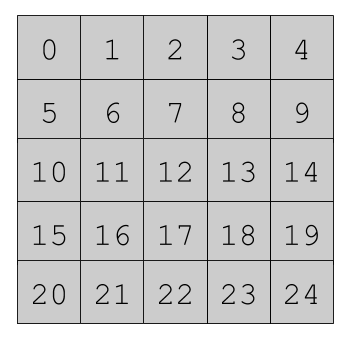
\includegraphics[scale = 0.5]{img/RedNumber.png}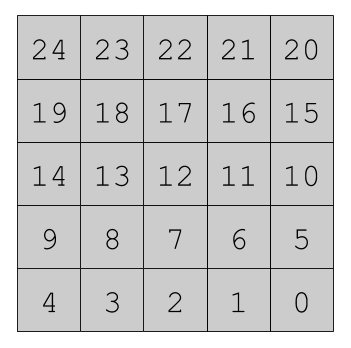
\includegraphics[scale = 0.5]{img/BlueNumber.png}

        舉例來說:以下的兩個盤面雖然輪到的人不同,棋盤的樣子也不一樣,但它們的四種棋子的位置分佈都相同,因此可以視為等價。

        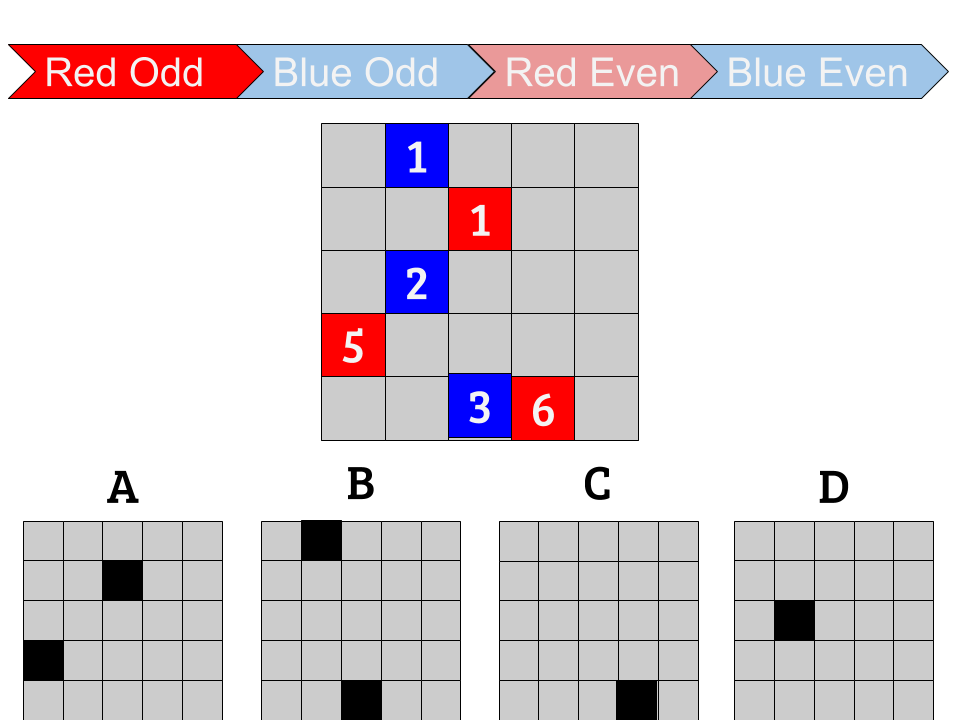
\includegraphics[scale=0.25]{img/Board1}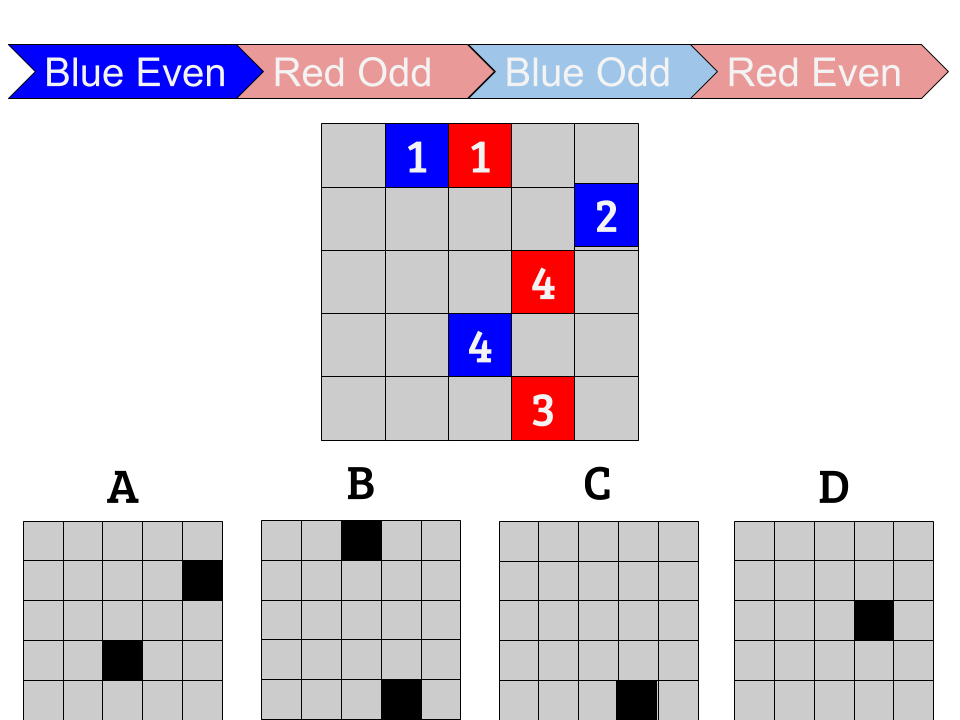
\includegraphics[scale=0.25]{img/Board2}\\
        \(A = \{7, 15\}\)\\
        \(B = \{1, 22\}\)\\
        \(C = \{23\}\)\\
        \(D = \{11\}\)\\
        我的編碼方式是先把 \(A\), \(B\), \(C\), \(D\) 分別以上述的順序轉換成一個長度為 25 的 bitset,再把這四個 bitset 接起來,形成一個長度為 100 的 bitset。\\
        \(Enc(A) = 0000000001000000010000000\)\\
        \(Enc(B) = 0010000000000000000000010\)\\
        \(Enc(C) = 0100000000000000000000000\)\\
        \(Enc(D) = 0000000000000100000000000\)\\
        \(Enc(\text{Board})=Enc(D)Enc(C)Enc(B)Enc(A)\)\\
        Board 在一手之後的盤面會是 \(Enc(A')Enc(D')Enc(C')Enc(B')\)。
    \subsection{Information Storage}
        我建立了一個 \texttt{bitset -> pair<double, double>} 的 hash table \texttt{trans},一個盤面的勝場數和敗場數會被紀錄在 \texttt{trans[}\(Enc(\text{Board})\)\texttt{]}中。
    \subsection{Searching Strategy}
        定義 \(Move(Enc(\text{board}))=\{Enc(\text{all possible board after one move})\}\).
        採用 \textit{Monte-Carlo Tree Search},並對勝/敗場數的平均與標準差以 \textit{Progressive Pruning} 作為優化。\(Enc(\text{board})\)的小孩是所有 \(Move(Enc(\text{board}))\) 內的元素。由於 \(Enc\) 的編號是以「該回合的玩家」為標準,造成的效果就像是每一手都把盤面旋轉 180 度。因此我的作法比起 Min-Max,更像是 Nega-Max。
    \subsection{Parameters}
    \begin{itemize}
        \item Simulating times per child when expanding: \(100\)
        \item \(r_d\): \(2.0\)
        \item \(\sigma_e\): \(0.2\)
    \end{itemize}
\end{document}
